\documentclass{article}

\usepackage{circuitikz}
\usepackage[T1]{fontenc} 
\usepackage[UTF8]{inputenc}
\usepackage{amsmath}
\usepackage{amssymb}
\usepackage{fancyhdr}
\usepackage{graphicx}
\usepackage{hyperref}
\usepackage{tikz}
  \usetikzlibrary{arrows}
  \usetikzlibrary{shapes}
  \usetikzlibrary{arrows.meta,topaths}
  \usetikzlibrary{bending}
  \usetikzlibrary{calc}
\usepackage{anyfontsize}
\usepackage{sectsty}
\usepackage{../assets/scripts/tex/color-env}
\usepackage{anyfontsize}
\usepackage{xcolor}
\definecolor{DarkGreenBlue}{HTML}{264653}
\definecolor{LightGreenBlue}{HTML}{2A9D8F}
\definecolor{LightOrange}{HTML}{E9C46A}
\definecolor{DarkOrange}{HTML}{F4A261}
\definecolor{RedOrange}{HTML}{E76F51}
\definecolor{BrightRed}{HTML}{D62828}
\definecolor{DeepBlue}{HTML}{003049}



\usepackage[ngerman]{babel}
\title{Elektrotechnik 1 - Praktikum 3}


\usepackage[
  includehead,
  headheight = 17mm,
  footskip = \dimexpr\headsep+\ht\strutbox\relax,
  tmargin = 0mm,
  bmargin = \dimexpr17mm+2\ht\strutbox\relax,
]{geometry}





\pagestyle{fancy}
\fancyhead[L]{\leftmark}
\fancyhead[R]{}
\fancyfoot[L]{}
\fancyfoot[C]{\thepage}
\fancyfoot[R]{
\includegraphics[scale=0.2]{../assets/images/haw.jpg}}
\renewcommand\headrulewidth{0.5pt}


\begin{document}


\thispagestyle{empty}
\begin{tikzpicture}[remember picture,overlay]

  \fill[DeepBlue] (current page.south west) rectangle (current page.north east);

  \begin{scope}

    \foreach \i in {2.5,...,22}
      {
        \node[rounded corners, DeepBlue!90,draw ,regular polygon, regular polygon sides=6, minimum size=\i cm, ultra thick] at ($(current page.west)+(2.5,-5)$) {} ;
      }

  \end{scope}

  \node[rounded corners,fill=DeepBlue!95,text =DeepBlue!5,regular polygon,regular polygon sides=6, minimum size=2.5 cm,inner sep=0,ultra thick] at ($(current page.west)+(2.5,-5)$) {\LARGE \bfseries 2020};

  \foreach \i in {0.5,...,22}
    {
      \node[rounded corners,DeepBlue!90,draw,regular polygon,regular polygon sides=6, minimum size=\i cm,ultra thick] at ($(current page.north west)+(2.5,0)$) {} ;
    }

  \foreach \i in {0.5,...,22}
    {
      \node[rounded corners,DeepBlue!98,draw,regular polygon,regular polygon sides=6, minimum size=\i cm,ultra thick] at ($(current page.north east)+(0,-9.5)$) {} ;
    }

  \foreach \i in {12}
    {
      \node[fill = DeepBlue,rounded corners,draw=DeepBlue,regular polygon,regular polygon sides=6, minimum size=\i cm,ultra thick] at ($(current page.south east)+(-0.2,-0.45)$) {} ;
    }


  \foreach \i in {21,...,6}
    {
      \node[DeepBlue!95,rounded corners,draw,regular polygon,regular polygon sides=6, minimum size=\i cm,ultra thick] at ($(current page.south east)+(-0.2,-0.45)$) {} ;
    }

  \node[left,DeepBlue!5,minimum width=0.625*\paperwidth,minimum height=3cm, rounded corners] at ($(current page.north east)+(0,-9.5)$){{\fontsize{25}{30} \selectfont \bfseries ET2 - Praktikum 5}};

  \node[left,DeepBlue!10,minimum width=0.625*\paperwidth,minimum height=2cm, rounded corners] at ($(current page.north east)+(0,-11)$){{\huge \textit{Resonanz}}};

  \node[left,DeepBlue!5,minimum width=0.625*\paperwidth,minimum height=2cm, rounded corners] at ($(current page.north east)+(0,-13)$){{\Large \textsc{Florian Tietjen\hspace{0.5cm}Eric Antosch}}};

\end{tikzpicture}

\newpage
\thispagestyle{empty}

\tableofcontents


\newpage


\section{Vorbereitung}
Als Vorbereitung der folgenden Versuche werden vorher einige Kenngrößen eines Serienresonanzkreies berechnet.
Die Serienschaltung besteht dabei aus einer Induktivität L = 100 mH und einem Gleichstrom-Drahtwiderstand $R_L = 10 \Omega$ . Der Sinus-Generator
hat einen Innenwiderstand von $R_i = 50\Omega$. Die angegebene Größe der Induktivität gilt nur für Frequenzen f < 1kHz.

\subsection{Berechnung der erforderlichen Kapazität}
Die Formel zur Berechnung der Resonanzfrequenz wird nach der Kapazität C umgestellt.
\begin{align*}
  \omega_r & = \frac{1}{\sqrt{LC}} \\
  C        & = \frac{1}{{w_r}^2L}
\end{align*}
Mit der Formel werden nun die Kapazitäten verschiedener Frequenzen ausgerechnet:

\begin{table}[h]
  \begin{center}
    \begin{tabular}{|c|c|c|c|c|c|}
      \hline
      Frequenz  & $100 Hz$     & $500Hz$      & $1kHz$    & $5kHz$    & $10kHz$  \\
      \hline
      Kapazität & $25,33\mu F$ & $1,013\mu F$ & $253,3nF$ & $1,013nF$ & $2,53nF$ \\
      \hline
    \end{tabular}
    \caption{Berechnete Kapazitätswerte in Abhängigkeit von einer festen Frequenz}
    \label{tab:cFC}
  \end{center}
\end{table}

\subsection{Berechnung der Gütefaktoren und Bandbreiten}
Nun werden die zugehörigen Gütefaktoren Q und Bandbreiten $\Delta$f für jeweils den Gesamtverlustwiderstand R$_i$ + R$_L$ und den Spulen-Drahtwiderstand R$_L$ allein berechnet.
Für den Gesamtverlustwiderstand gilt:
\begin{align*}
  R_{ges} & = R_i + R_L= 50\Omega + 10\Omega = 60\Omega
\end{align*}
Die Formel der Güte einer Serienschaltung lautet:
\begin{align*}
  Q & = \frac{1}{R}\cdot\sqrt{\frac{L}{C}}
\end{align*}
Für die Bandbreite $\Delta$f ermittelt sich aus:
\begin{align*}
  B & = \frac{f_r}{Q}
\end{align*}
Für verschiedene Frequenzen ergeben sich dann folgende Güten und Bandbreiten:
\begin{table}[h]

  \begin{center}

    \begin{tabular}{|c|c|c|c|c|c|}
      \hline
      Freqeunz             & $100 Hz$     & $500Hz$      & $1kHz$    & $5kHz$    & $10kHz$  \\
      \hline
      $Q_{R_{ges}}$        & $25,33\mu F$ & $1,013\mu F$ & $253,3nF$ & $1,013nF$ & $2,53nF$ \\
      \hline
      $Q_L$                & $100 Hz$     & $500Hz$      & $1kHz$    & $5kHz$    & $10kHz$  \\
      \hline
      $\Delta f_{R_{ges}}$ & $25,33\mu F$ & $1,013\mu F$ & $253,3nF$ & $1,013nF$ & $2,53nF$ \\
      \hline
      $\Delta f_L$         & $25,33\mu F$ & $1,013\mu F$ & $253,3nF$ & $1,013nF$ & $2,53nF$ \\
      \hline
    \end{tabular}
    \caption{Güte und Bandbreite in Abhängigkeit von dem betrachtetem Widerstand und der Frequenz}
    \label{tab:cGB}
  \end{center}
\end{table}



\newpage

\section{Resonanz - Eingeschwungener Zustand}
\subsection{Versuch 1}
\begin{task}
  IIm ersten Versuch soll der Amplitudengang von $\hat{u}_C$ in der abgebildeten Schaltung mit dem Oszilloskop ermittelt werden. Dazu soll beachtet werden,
  dass $R_i = 50\Omega$ und $\hat{u}_{gen} = 1V$ sind. Die Kapazitätsdekade wird mit den berechneten Werten aus der Vorbereitung eingestellt.
\end{task}

\begin{figure}[h]
  \begin{center}
    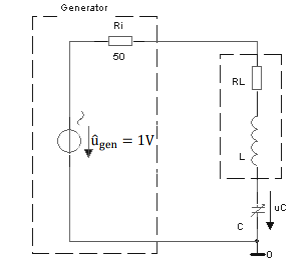
\includegraphics{../assets/images/ETP3/Versuch1Schaltplan.PNG}
    \caption{Schaltplan zum ersten Versuch der ersten Aufgaben zur Bestimmung des Spannungsverhältnisses $\frac{\hat{u}_C}{\hat{u}_{gen}}$}
  \end{center}
\end{figure}

\begin{devlist}
  T
  \begin{itemize}
    \item Oszilloskop: Tektronix MDO3012
    \item Funktionsgenerator: Keysight 33210A
    \item HP 4294A Impedance Analyzer
    \item Multimeter: MetraHit X-TRA Multimeter
  \end{itemize}
\end{devlist}

\newpage

\subsubsection{Bestimmung von $\frac{\hat{u}_C}{\hat{u}_{gen}}$}

\begin{table}[h]
  \begin{center}

    \begin{tabular}{|c|c|c|}
      \hline
          & $500Hz; C=1,01\mu F$ & $1kHz; C= 253,3 nF$ \\
      \hline
      -95 &                      &                     \\
      \hline
      -50 &                      &                     \\
      \hline
      -40 &                      &                     \\
      \hline
      -20 &                      &                     \\
      \hline
      -10 &                      &                     \\
      \hline
      -5  &                      &                     \\
      \hline
      0   &                      &                     \\
      \hline
      5   &                      &                     \\
      \hline
      10  &                      &                     \\
      \hline
      20  &                      &                     \\
      \hline
      40  &                      &                     \\
      \hline
      50  &                      &                     \\
      \hline
      95  &                      &                     \\
      \hline
    \end{tabular}
    \caption{Messwerte für Versuch 1.1}
    \label{tab:MV}
  \end{center}
\end{table}

\subsubsection{Graphische Darstellung der Ergebnisse}

\subsubsection{Ermittlung der Güte und der Bandbreite}

\begin{table}[h]
  \begin{center}
    \begin{tabular}{|c|c|c|}
      \hline
      Resonanzfrequenz &  & \\
      \hline
      Q                &  & \\
      \hline
      $\Delta$f        &  & \\
      \hline
    \end{tabular}
    \caption{Aus den Messwerten berechnete Güte und Bandbreite}
    \label{tab:eMGB}
  \end{center}
\end{table}
\newpage
\subsection{Versuch 2}

\begin{task}
  IIm nächsten Abschnitt soll nun mithilfe eines Operationsverstärker-Impedanzwandlers
  der Innenwiderstand des Generators abgekoppelt werden. Um keine Verzerrungen bei der Erfassung
  des Signals zu bekommen, ist es hilfreich die Generatorspannung $\hat{u}_{gen}$ geringer zu wählen.
\end{task}
\begin{figure}[h]
  \begin{center}
    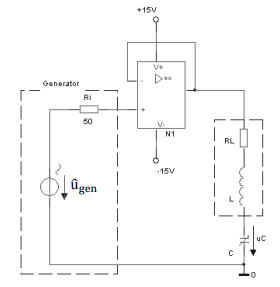
\includegraphics{../assets/images/ETP3/Versuch2Schaltplan.PNG}
    \caption{Schaltplan für den zweiten Versuch mit Operationsverstärker-Impedanzwandler}
  \end{center}
\end{figure}

\begin{table}[h]
  \begin{center}

    \begin{tabular}{|c|c|c|c|c|}
      \hline
          & \multicolumn{2}{c|}{$500Hz; C=1,01\mu F$} & \multicolumn{2}{c|}{$1kHz; C= 253,3 nF$}                                                   \\
      \hline
          & $\hat{u}_C$                               & $\frac{\hat{u}_C}{\hat{u}_{gen}}$        & $\hat{u}_C$ & $\frac{\hat{u}_C}{\hat{u}_{gen}}$ \\
      \hline
      -95 &                                           &                                          &             &                                   \\
      \hline
      -50 &                                           &                                          &             &                                   \\
      \hline
      -40 &                                           &                                          &             &                                   \\
      \hline
      -20 &                                           &                                          &             &                                   \\
      \hline
      -10 &                                           &                                          &             &                                   \\
      \hline
      -5  &                                           &                                          &             &                                   \\
      \hline
      0   &                                           &                                          &             &                                   \\
      \hline
      5   &                                           &                                          &             &                                   \\
      \hline
      10  &                                           &                                          &             &                                   \\
      \hline
      20  &                                           &                                          &             &                                   \\
      \hline
      40  &                                           &                                          &             &                                   \\
      \hline
      50  &                                           &                                          &             &                                   \\
      \hline
      95  &                                           &                                          &             &                                   \\
      \hline
    \end{tabular}
    \caption{Messwerte für Versuch 2}
    \label{tab:MV2}
  \end{center}
\end{table}

\subsubsection{Graphische Darstellung}

\subsubsection{Berechnung der Güte und der Bandbreite}

\begin{table}[h!]
  \begin{center}
    \begin{tabular}{|c|c|c|}
      \hline
      Resonanzfrequenz &  & \\
      \hline
      Q                &  & \\
      \hline
      $\Delta$f        &  & \\
      \hline
    \end{tabular}
    \caption{Aus den Messwerten berechnete Güte und Bandbreite}
    \label{tab:zMGB}
  \end{center}
\end{table}

\subsection{Vergleich}


\subsection{Versuch mit höheren Resonanzfrequenzen}

\begin{table}[h]

  \begin{center}

    \begin{tabular}{|c|c|c|c|c|}
      \hline $\mathrm{f}$       & $\mathrm{C}$        & $\hat{u}_{g e n}$ & $\hat{u}_C$       & $\mathrm{Q}$ \\
      \hline $5 \mathrm{kH} z$  & $10,13 \mathrm{nF}$ & $166 \mathrm{mV}$ & $4,00 \mathrm{V}$ & 24,1         \\
      \hline $10 \mathrm{kH} z$ & $2,53 \mathrm{nF}$  & $166 \mathrm{mV}$ & $3,2 \mathrm{V}$  & 19,28        \\
      \hline
    \end{tabular}
    \caption{Ergebnis aus der Testreihe mit höheren Frequenzen}
    \label{tab:lCUQ}
  \end{center}
\end{table}
$$Q=\frac{1}{R} \cdot \sqrt{\frac{L}{C}} \Leftrightarrow R=\frac{1}{Q} \cdot \sqrt{\frac{L}{C}}$$
\begin{equation*}
  \text { Bei } f=5 k H z: \quad R=\frac{1}{24,1} \cdot \sqrt{\frac{100 m H}{10,13 n F}}=130,37 \Omega
\end{equation*}
\begin{equation*}
  \text { Bei } f=10 \mathrm{kHz}: \quad R=\frac{1}{19,28} \cdot \sqrt{\frac{100 \mathrm{mH}}{2,53 \mathrm{nF}}}=326,1 \Omega
\end{equation*}

\newpage
\section{Resonanz - Schaltverhalten}
\begin{task}
  IIn diesem Versuch wird wieder die Schaltung aus 1.1 aufgebaut. Für die Messungen wird zwischen dem Generator und der Spule/C-Dekade eine Präzisions-Widerstandsdekade verschaltet.
  Die Kreisresonanz wird mit der C-Dekade auf f = 1kHz eingestellt. An die Schaltung wird eine symmetrische Rechteckspannung mit einer Frequenz f = 50Hz, Tastverhältnis a = 0,5 und einem Scheitelwert von $\hat{u}_{gen} = 1,0 V$ angelegt.
  Der zeitliche Verlauf der Spannung am Kondensator wird mittels Oszilloskop dargestellt
\end{task}

\begin{devlist}
  T
  \begin{itemize}
    \item Oszilloskop: Tektronix MDO3012
    \item Kapazitätsdekade Time Electronics Model 1071 CapBox
    \item Funktionsgenerator: Keysight 33210A
    \item Multimeter: MetraHit X-TRA Multimeter
  \end{itemize}
\end{devlist}

\subsection{Serienschwingkreis mit Dämpfung}

Abbildung gedämpfter Schwingkreis\\\\

Messwerte:
\begin{table}[h]
  \begin{center}

    \begin{tabular}{|c|c|c|c|}
      \hline
      $T_d$  & $\overline{u}$ & $y_i$   & $y_{i+1}$ \\
      \hline
      ca 1ms & ca -1v         & ca860mV & ca340mV   \\
      \hline
    \end{tabular}
  \end{center}
\end{table}
Berechnung des Dämpfungsmaß:
\begin{align*}
  \delta   & = \frac{1}{T_d} \cdot \ln \left(\frac{Y_i}{Y_{i+1}}\right)                                \\
  \omega   & = 2\pi \cdot f = 2\pi \cdot \frac{1}{T_d} = hier muss ca das gleiche wie unten rauskommen \\
  \omega_r & = \frac{1}{\sqrt{LC}} = \frac{1}{\sqrt{100mH \cdot 253,3nF}} = 6283 s^{-1}
\end{align*}


\subsection{Aperiodischer Grenzfall}

Abbildung Aperiodischer Grenzfall

Wert liegt circa bei 1,0753k Ohm

\end{document}